\chapter{Evaluation}
For my evaluation, I've used {\bf Tensorboard} for plotting the learning(loss) curve and performance(accuracy) curve for both training and validating processes. Also, I've used external open source library({\bf pretty-print-confusion-matrix}\footnote{\url{https://github.com/wcipriano/pretty-print-confusion-matrix}}) for plotting the confusion matrix for the test set.

In all the plots, x-axis corresponds to the epoch.
As for the graphs,

\begin{itemize}
\item Accuracy graph
	\begin{itemize}
	\item Dark red: train accuracy
	\item Bright red: validation accuracy
	\end{itemize}

\item Loss graph
	\begin{itemize}
	\item Dark blue: train loss
	\item Bright blue: validation loss
	\end{itemize}
\end{itemize}

\newpage
\section{Original model}

\begin{figure}[htbp]
\centering
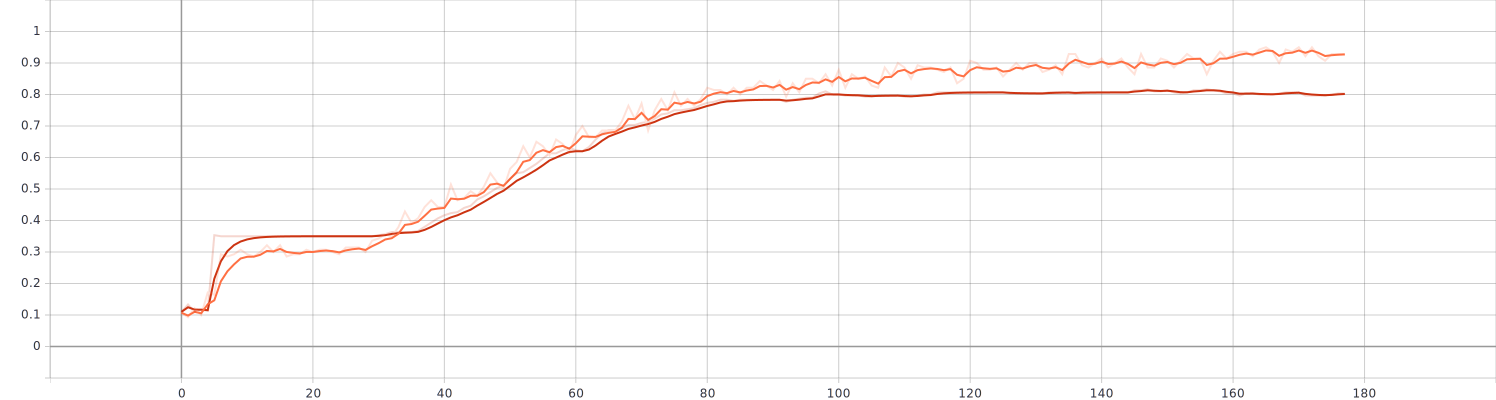
\includegraphics[width=0.7\linewidth]{evaluation/fig/Accuracy0.png}
\caption{Accuracy graph}
\label{fig:accuracy0}
\end{figure}

\begin{figure}[htbp]
\centering
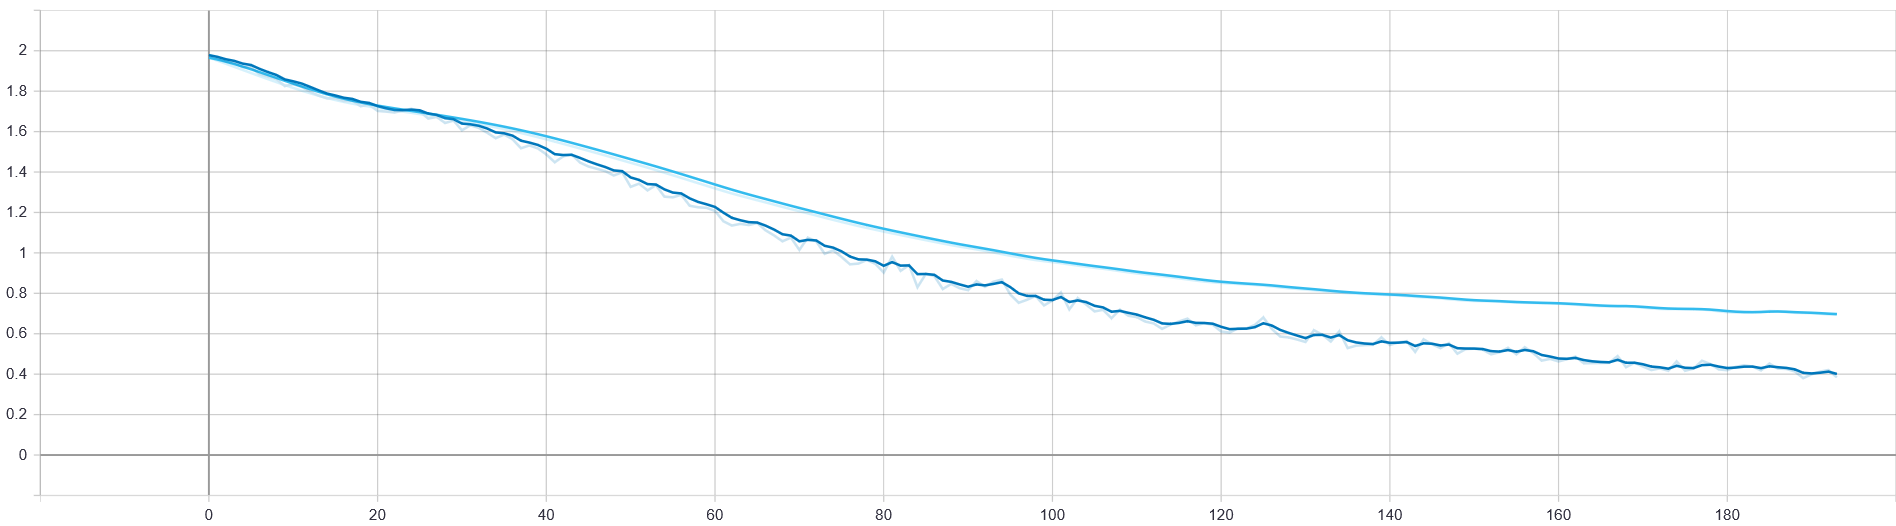
\includegraphics[width=0.7\linewidth]{evaluation/fig/Loss0.png}
\caption{Loss graph}
\label{fig:evaluation0}
\end{figure}

\begin{figure}[htbp]
\centering
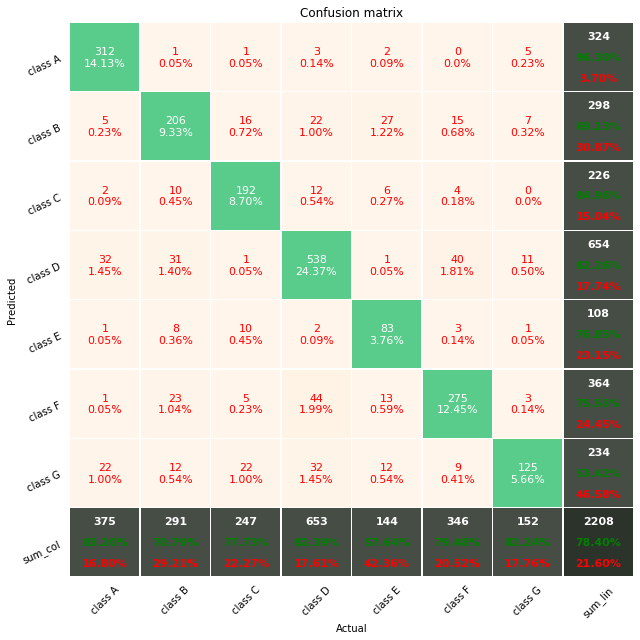
\includegraphics[width=0.6\linewidth]{evaluation/fig/confusion0.png}
\caption{Confusion matrix}
\label{fig:confusion0}
\end{figure}

\newpage
\section{Modified Model (Ver. 1)}

\begin{figure}[htbp]
\centering
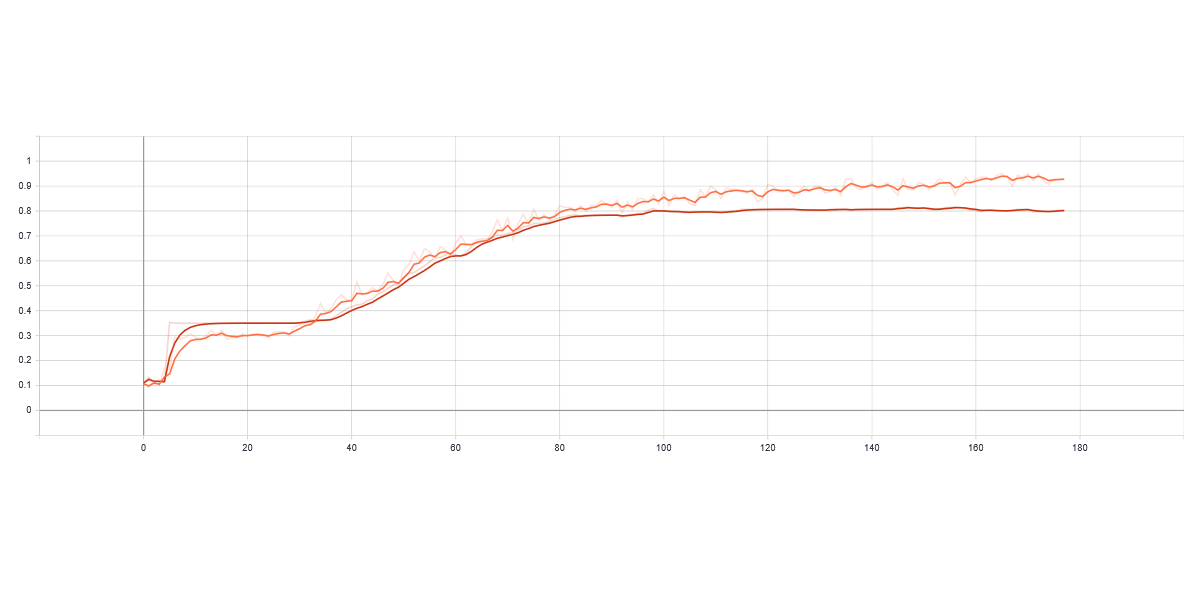
\includegraphics[width=0.7\linewidth]{evaluation/fig/Accuracy1.png}
\caption{Accuracy graph}
\label{fig:accuracy1}
\end{figure}

\begin{figure}[htbp]
\centering
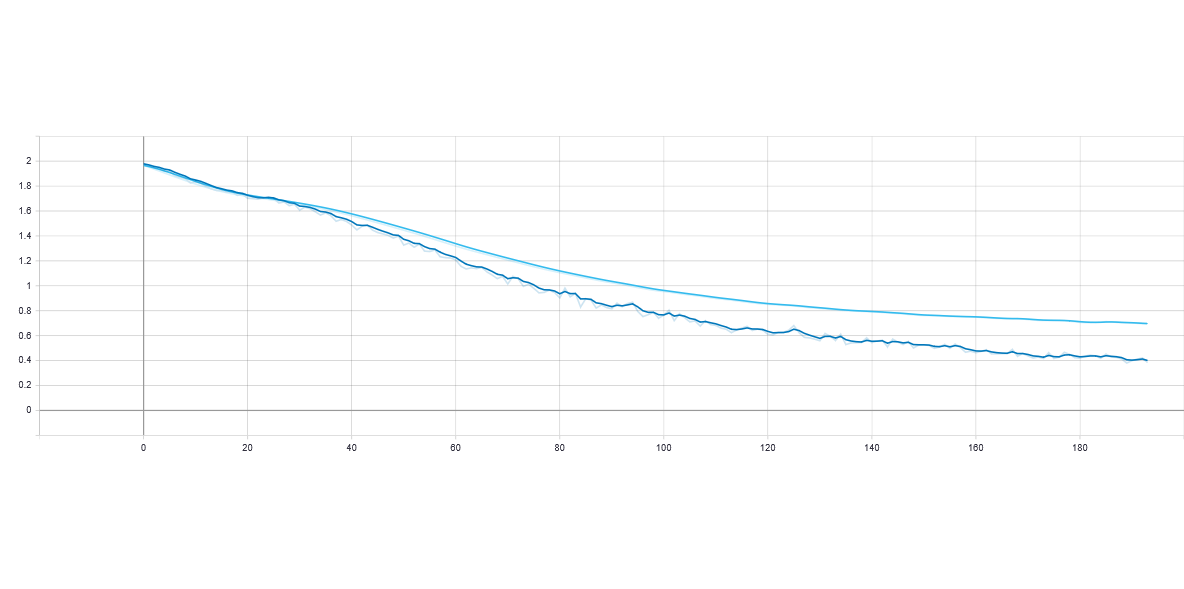
\includegraphics[width=0.7\linewidth]{evaluation/fig/Loss1.png}
\caption{Loss graph}
\label{fig:evaluation1}
\end{figure}

\begin{figure}[htbp]
\centering
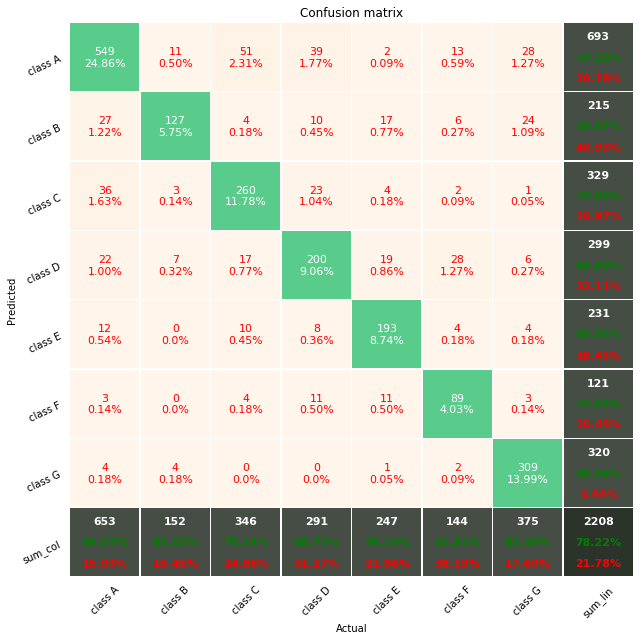
\includegraphics[width=0.6\linewidth]{evaluation/fig/confusion1.png}
\caption{Confusion matrix}
\label{fig:confusion1}
\end{figure}

\newpage
\section{Modified Model (Ver. 2)}

\begin{figure}[htbp]
\centering
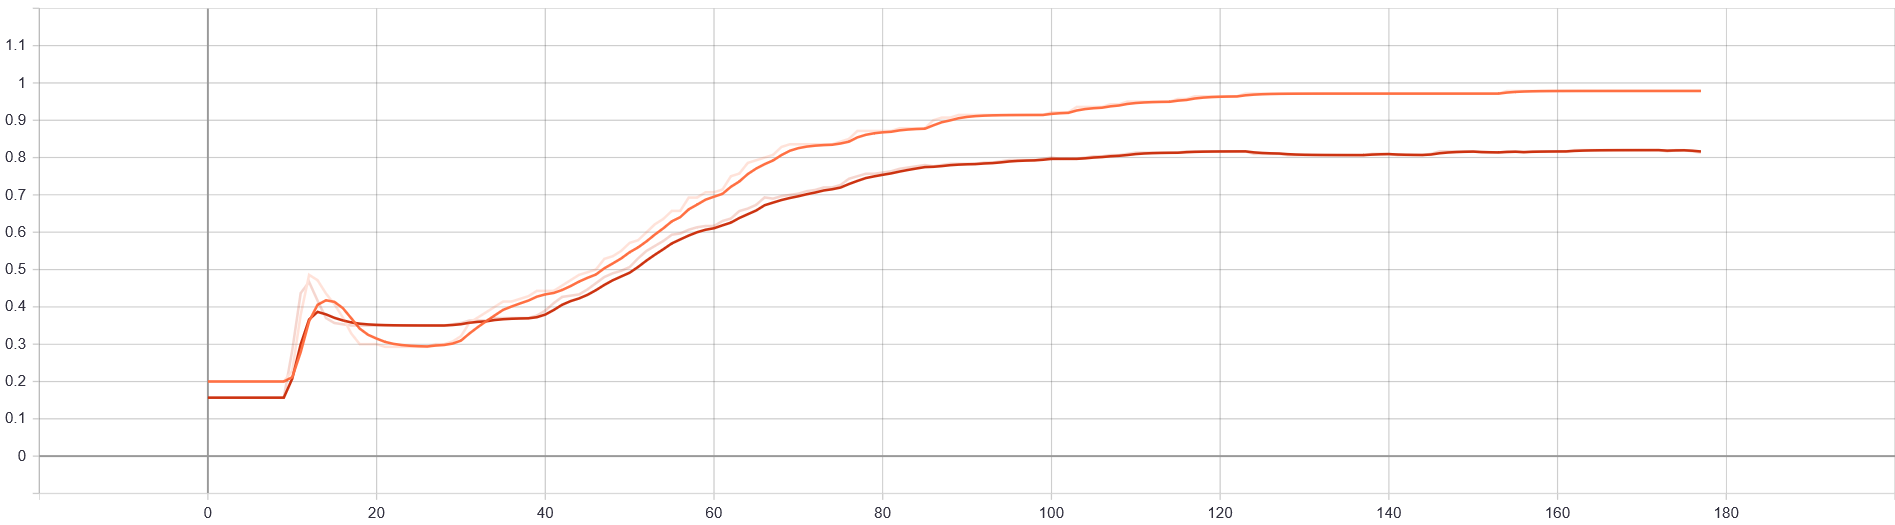
\includegraphics[width=0.7\linewidth]{evaluation/fig/Accuracy2.png}
\caption{Accuracy graph}
\label{fig:accuracy2}
\end{figure}

\begin{figure}[htbp]
\centering
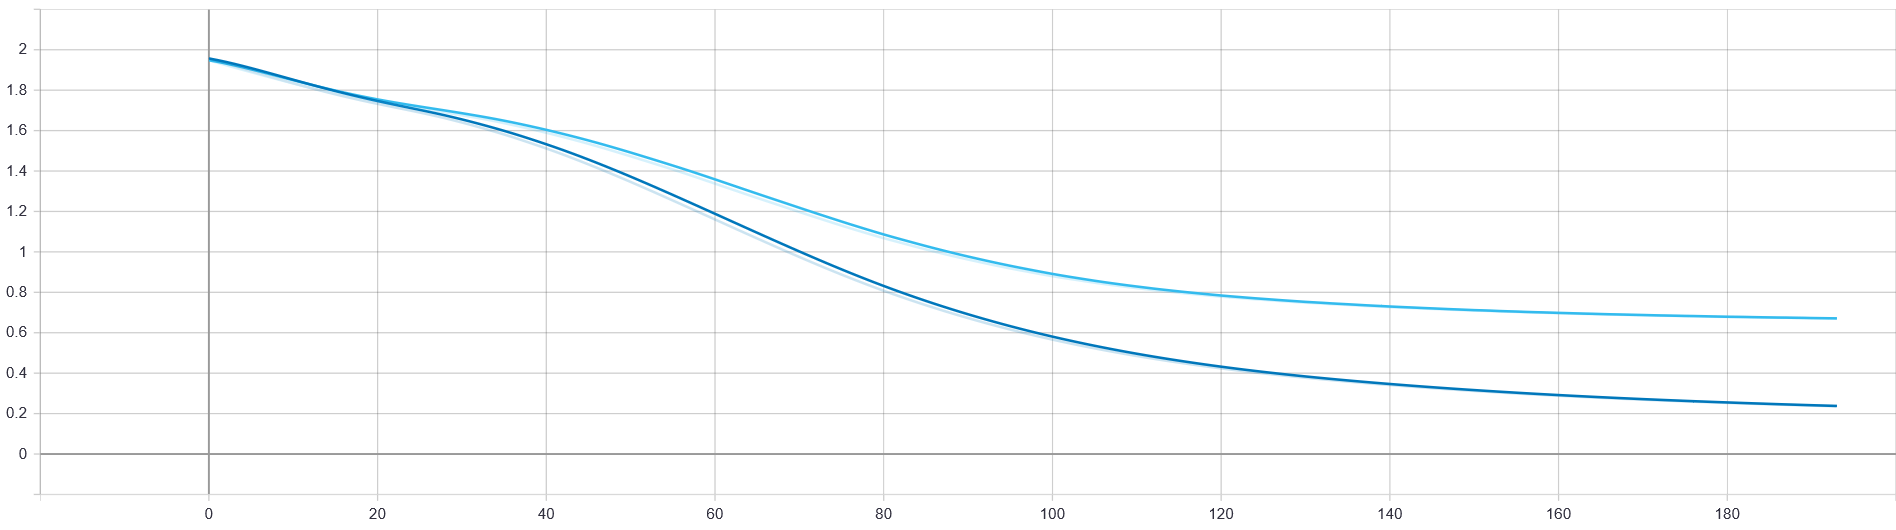
\includegraphics[width=0.7\linewidth]{evaluation/fig/Loss2.png}
\caption{Loss graph}
\label{fig:evaluation2}
\end{figure}

\begin{figure}[htbp]
\centering
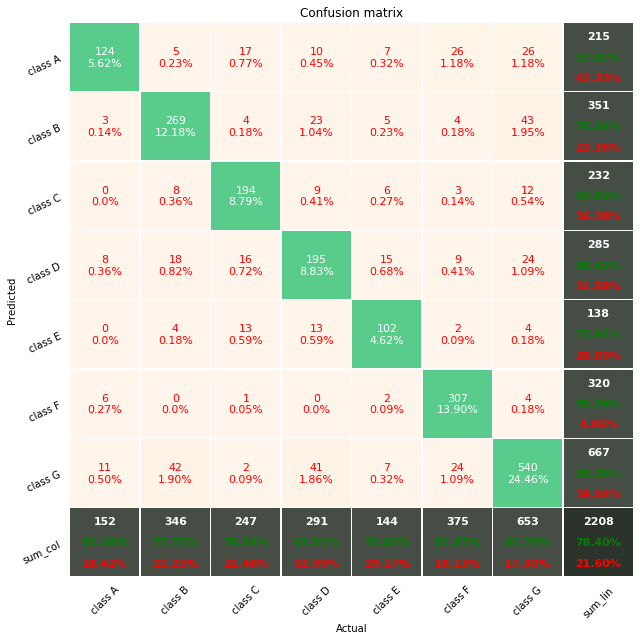
\includegraphics[width=0.6\linewidth]{evaluation/fig/confusion2.png}
\caption{Confusion matrix}
\label{fig:confusion2}
\end{figure}

\newpage
\section{Modified Model (Ver. 3)}

\begin{figure}[htbp]
\centering
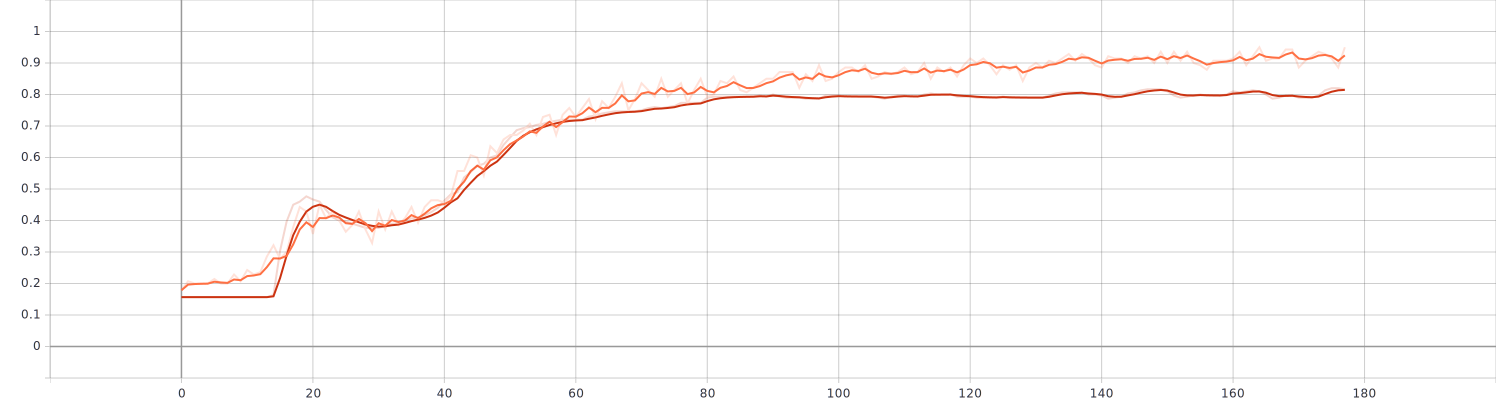
\includegraphics[width=0.7\linewidth]{evaluation/fig/Accuracy3.png}
\caption{Accuracy graph}
\label{fig:accuracy3}
\end{figure}

\begin{figure}[htbp]
\centering
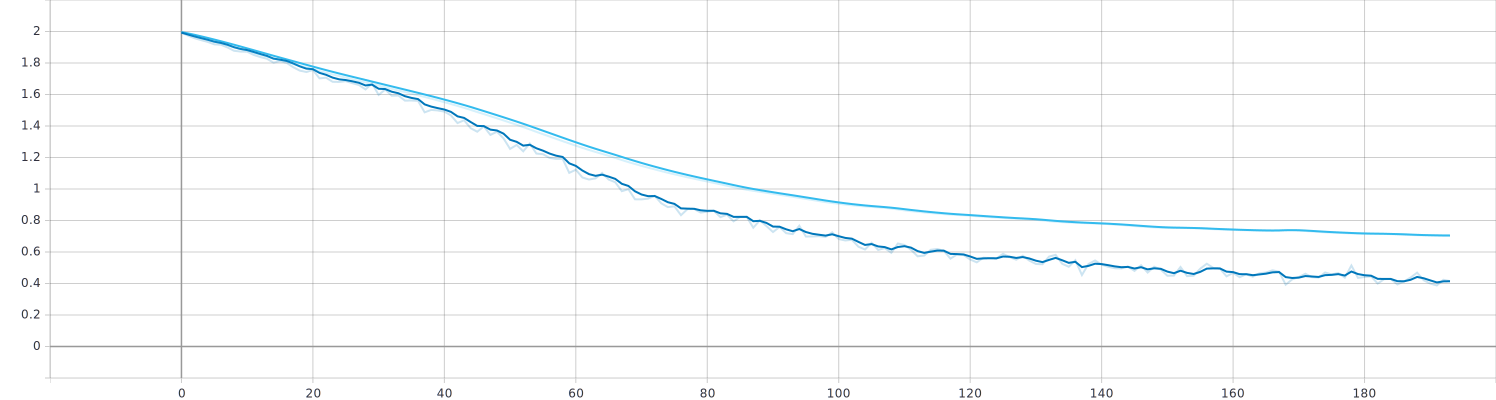
\includegraphics[width=0.7\linewidth]{evaluation/fig/Loss3.png}
\caption{Loss graph}
\label{fig:evaluation3}
\end{figure}

\begin{figure}[htbp]
\centering
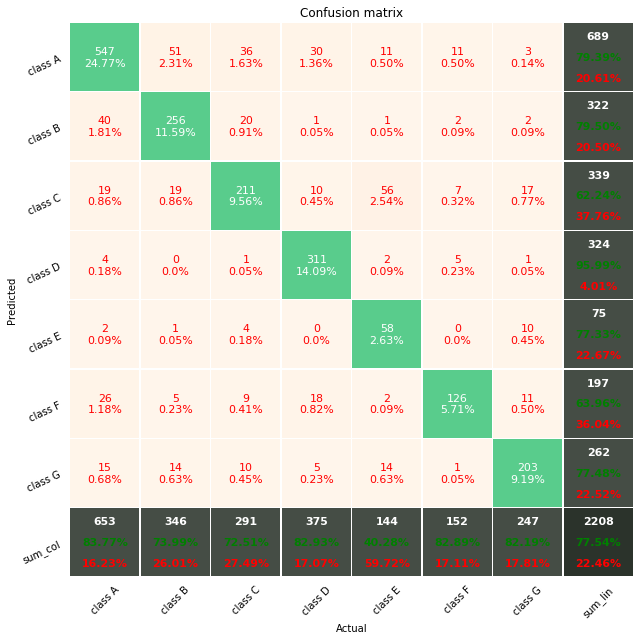
\includegraphics[width=0.6\linewidth]{evaluation/fig/confusion3.png}
\caption{Confusion matrix}
\label{fig:confusion3}
\end{figure}
